\section{Flexibility in PSWare}
\label{sec:flexibility}
In this section, we discuss how PSWare can achieve the desired flexibility in different aspects of an event-based system, including, event detection, event delivery and event subscription.

\subsection{Flexibility in Event Detection}
Event detection is the heart of an event-based system. In PSWare, we can easily customize the event detection algorithm by using the middleware framework.

We demonstrate the flexibility in event detection through an example in this subsection. The example is TED \cite{lai:ted}, the default event detection algorithm used by PSWare. TED aims at minimizing energy consumption. %The second example is 

\begin{figure}
\centering
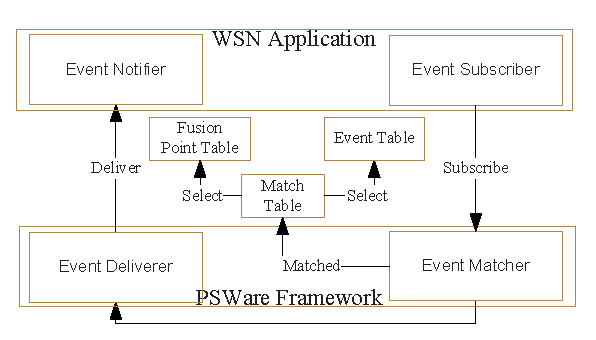
\includegraphics[width=.8\textwidth]{ted-architecture}
\caption{TED over PSWare}
\label{fig:ted-architecture}
\end{figure}

The essential idea of TED is fusion point selection, where the sensor nodes detect events and select parent nodes according to the detection cost so that the cost for future event detection can be reduced. The interaction between TED, PSWare and the upper level application is shown in Figure \ref{fig:ted-architecture}.

To implement TED in PSWare, we use three sub-procedures that can support the major functionality of TED:
\begin{enumerate}
\item A procedure for each of the nodes to exchange their information about available fusion points (fusion point table in Figure \ref{fig:ted-architecture}). This procedure is executed periodically and is independent of event detection.
\item A procedure for each of the nodes to exchange their information about the detected events (event table in Figure \ref{fig:ted-architecture}). This procedure is also executed periodically and is independent of event detection.
\item A procedure that implements event matching interface as discussed in Section \ref{sec:model}, Listing \ref{lst:pswareEventMatcher}. This procedure is invoked during event matching.
\end{enumerate}

\begin{algorithm}
\begin{algorithmic}
\REQUIRE \(v_n\rightarrow msg_r\)
	\FOR {each entry \(t'\) in \(msg_r\)}
		\IF {\NOT exists \(t'\rightarrow fid_n\) in \(table_r\)}
			\STATE \(addTo(table_r, t')\)
		\ENDIF
		\FOR {each entry \(t\) in \(table_r\)}
			\IF {\(t\rightarrow fid_n = t'\rightarrow f_n\)}
				\IF {\(t'\rightarrow hop_n < t\rightarrow hop_n\)}
					\STATE \(t\rightarrow hop_n \gets t\rightarrow hop_n+1\)
					\STATE \(t\rightarrow parent_n \gets v_n\)
				\ENDIF
			\ENDIF
		\ENDFOR
	\ENDFOR
	\IF {self is fusion point \AND \NOT exists \(self\rightarrow id\) in \(table_r\)}
		\STATE \(addTo(table_r, (self\rightarrow id, 0, self\rightarrow id))\)
	\ENDIF
	\STATE \(msg_r \gets table_r\)
	\STATE \(periodically\_broadcast(msg_r)\)
\end{algorithmic}
\caption{Fusion point table exchange}
\label{algo:table_r}
\end{algorithm}

To illustrate the implementation, we briefly introduce some notations used by TED. In TED, some of the nodes \(V'\subseteq V\) in the network are selected as event fusion points. Each individual sensor node maintains a fusion point table \(table_r\) for all \(v'_n\in V'\)
\begin{itemize}
\item Fusion point ID (\(fid_n\)): the node ID of the fusion point
\item	Hop count (\(hop_n\)): the number of hops to reach the fusion point
\item	Parent (\(parent_n\)): the next hop to that fusion point
\end{itemize}
Each sensor node will also maintain an event table \(table_e\) containing the information for each event type \(e_n\in E\) which includes the following fields:
\begin{itemize}
\item Event type ID (\(e_n\)): the ID which is assigned to each event type
\item Fusion point for the event (\(fusion_n\)): the fusion point at which the event is mostly likely to be detected at the lowest cost.
\item Fusion cost (\(cost_n\)): the fusion cost for event type \(e_n\)
\end{itemize}
In addition to the above tables, each fusion point \(v'\in V'\) will maintain another table, the event matching \(table_m\) for the purpose of matching events. \(table_m\) contains the following fields:
\begin{itemize}
\item Event type ID (\(e_n\)): the ID of the event type
\item Event instance ID (\(i\)): the \(i\)th event instance of event type \(e_n\) (we use \(e_n^i\) to denote such an instance of event)
\item Source node (\(v_n^i\)): the node which forwarded \(e_n^i\) to the fusion point
\item Event timestamp (\(t_n^i\)): the timestamp when the event \(e_n^i\) is detected
\item Detection cost (\(cost_n^i\)): the cost for detecting event \(e_n^i\)
\end{itemize}

First, each node \(v_n\) periodically broadcasts messages \(msg_r\) which is its \(table_r\). If the node itself is a fusion point, then it will add itself in \(table_r\) and broadcast the message. The procedure is shown in Procedure \ref{algo:table_r}. In addition to \(msg_r\), each \(v'_k\in V'\) will periodically advertise its \(table_m\) by broadcasting \(msg_m\) so that other sensor nodes can construct their \(table_e\) with Procedure \ref{algo:table_e}.

\begin{algorithm}
\begin{algorithmic}
\REQUIRE \(v'_k\rightarrow msg_m\)
	\FOR {each entry \(t'\) in \(msg_m\)}
		\IF {\NOT exists \(t'\rightarrow e_n\) in \(table_e\)}
			\STATE \(addTo(table_e, (t'\rightarrow e_n, 1, v'_k, t'\rightarrow cost_n^i+table_r\rightarrow hop_k))\)
		\ENDIF
		\FOR {each entry \(t\) in \(table_e\)}
			\IF {\(t\rightarrow e_n = t'\rightarrow e_n\)}
				\IF {\(t'\rightarrow cost_n^i+table_r\rightarrow hop_k < t\rightarrow cost_n\)}
					\STATE \(t\rightarrow cost_n \gets t'\rightarrow cost_n^i+table_r\rightarrow hop_k\)
					\STATE \(t\rightarrow fusion_n \gets v'_k\)
				\ENDIF
			\ENDIF
		\ENDFOR
	\ENDFOR
	\IF {self is fusion point}
		\STATE \(msg_m \gets table_m\)
		\STATE \(periodically\_broadcast(msg_m)\)
	\ENDIF
\end{algorithmic}
\caption{Event table exchange}
\label{algo:table_e}
\end{algorithm}

The construction of \(table_m\) will take place when the event instance \(e_n^i\) is detected and forwarded to a fusion point \(v'_n\). We will discuss how forwarding could be done in the next subsection.

When an event \(e_n^i\) is matched at node \(v_k\), node will use \(table_r\) and \(table_e\) to decide how to forward the detected event to the fusion points so that higher level events can be matched. In case the fusion point for event type \(e_n\) has not been decided, the node will forward the event to some of its closet fusion points  according to TED. Upon the reception of \(e_n^i\) from \(v_k\), the fusion point will first update its own \(table_m\). Then it will check if there is any composite event \(e_{comp}\) which uses \(e_n\) and another event \(e_j\) as its sub-event (\(e_{comp}=comp(e_n, e_j)\)). If there is, then \(e_j\) will be used upon 'selectSubevent'.

\begin{algorithm}
\begin{algorithmic}
\REQUIRE \(e_n^i\) matched by \(v_k\) with cost: \(cost_n^i\)
	\STATE \(addTo(table_m, (e_n, e_n^i, v_k, now(), cost_n^i))\)
	\FOR {each \(e_j\) in \(E\)}
		\IF {\(\exists r\in R\) \AND \(r=e_{comp}=comp(e_n, e_j)\)}
			\FOR {each \(e_j^k\) in \(table_m\)}
				\IF {\(comp(e_n^i, e_j^k)=true\)}
					\STATE \(addTo(table_m, (e_{comp}, e_{comp}^i, self, now(), cost_n^i+cost_j^k))\)
					\STATE \(detected(e_{comp})\)
				\ENDIF
			\ENDFOR
		\ENDIF
	\ENDFOR
\end{algorithmic}
\caption{Event matching}
\label{algo:eventmatching}
\end{algorithm}

If \(e_{comp}\) has been successfully detected by the underlying event matcher, then Procedure \ref{algo:eventmatching} will be executed so that \(table_m\) is updated accordingly and TED may reduce the energy cost for future event detection.

\subsection{Flexibility in Event Delivery}
After the subscribed event is detected, it needs to be delivered to the user. In many applications, this is done via the underlying routing protocols such as CTP provided by TinyOS. This is also the case for the default event delivery in PSWare. However, in some applications, this may not be a case. For example, in an intelligent transportation system, the events may be delivered to mobile vehicles. In this subsection, we show how PSWare can achieve the flexibility in event delivery through several examples in ITS.

We choose ITS as an example because different event types in this application may require different event delivery strategies and that is why the flexibility in event delivery is of particular importance. The event types in ITS may include:
\begin{itemize}
\item Emergency: events that represent urgent incidents. Examples of this type of events include car accidents and urgent road maintenance. These events probably need to be delivered to all nearby vehicles when occurred.
\item Driver's information: events that provide assistant information to the drivers. Examples include congestion information and whether information These events are usually not considered as urgent and may be delivered in carry-and-forward fashion \cite{cartel}.
\end{itemize}

\begin{figure}
\centering
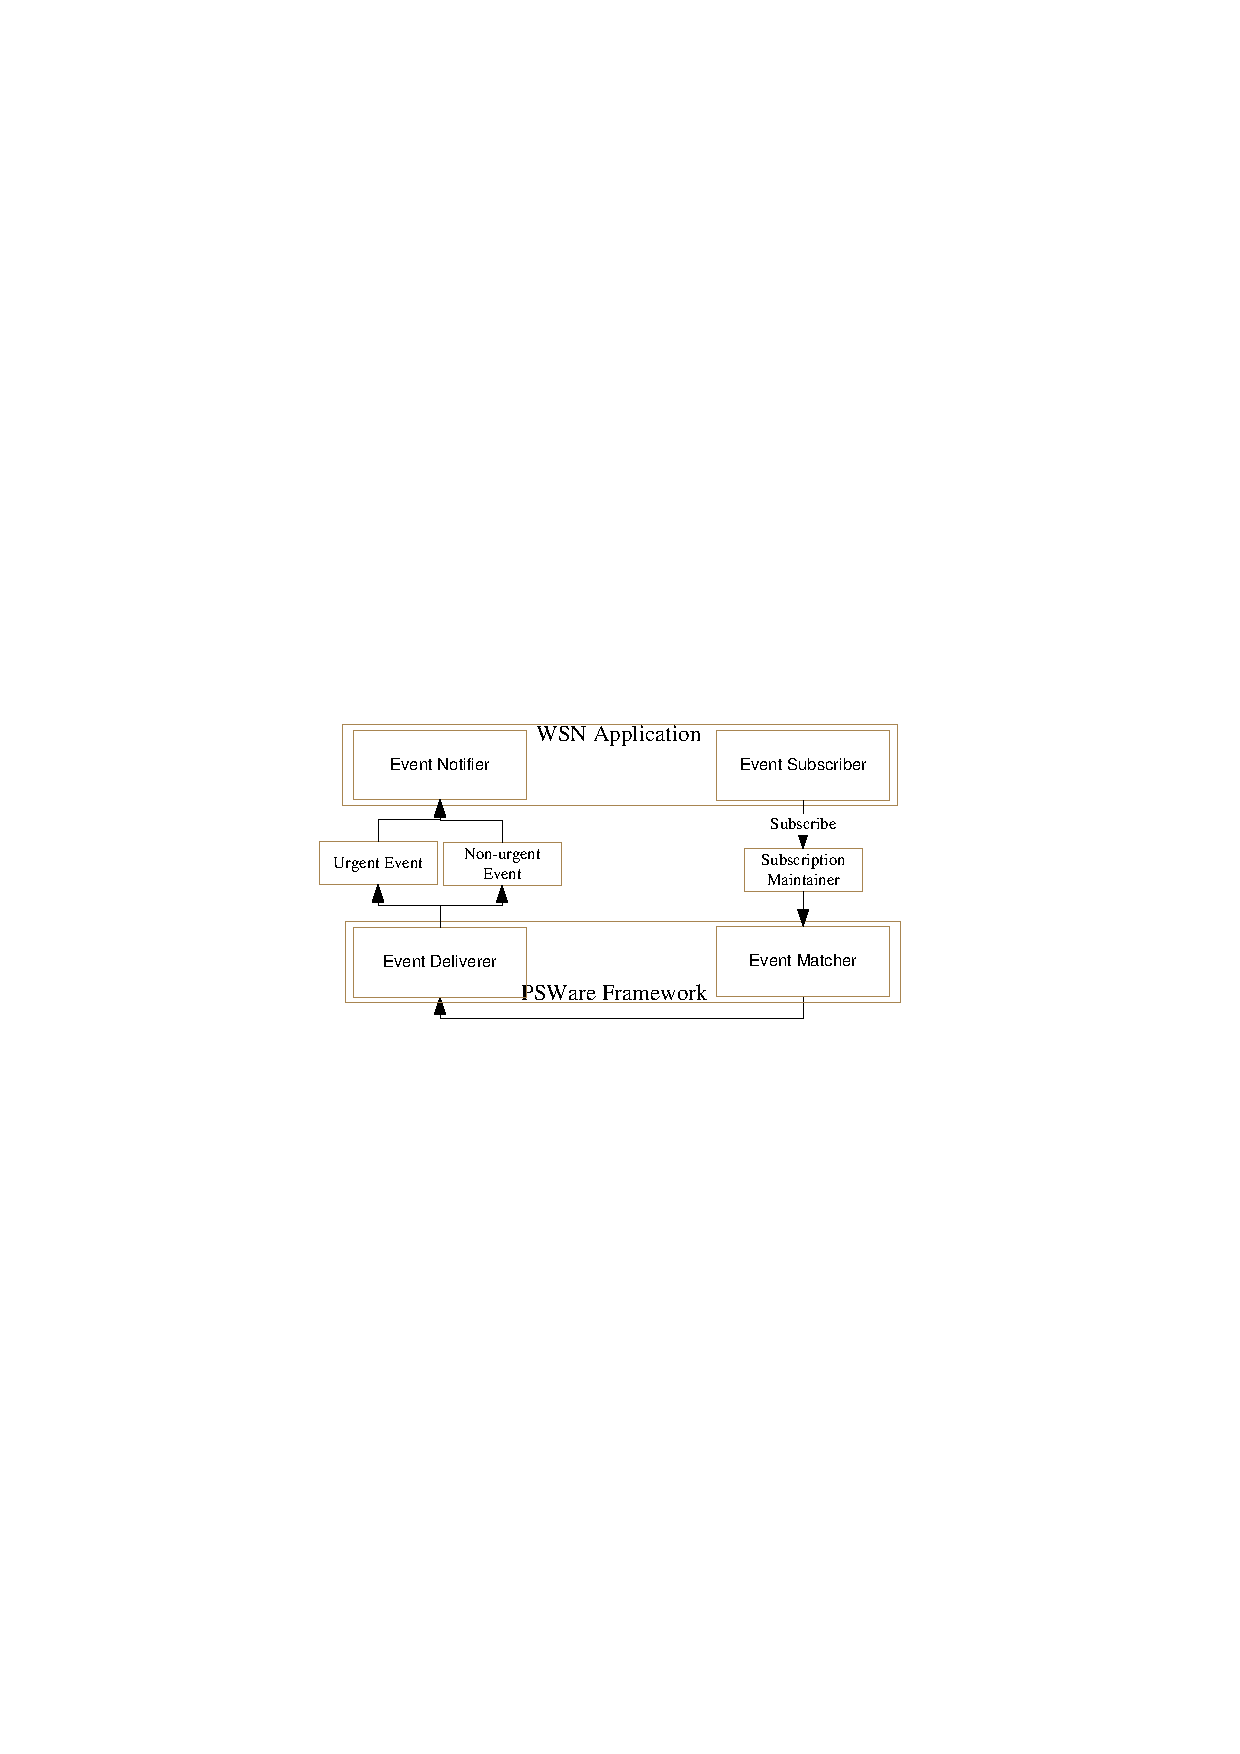
\includegraphics[width=.8\textwidth]{its-delivery}
\caption{Type-based event delivery}
\label{fig:its-delivery}
\end{figure}

The overall architecture for ITS event delivery over PSWare is shown in Figure \ref{fig:its-delivery}. A key difference in this architecture is the introduction of multiple event deliverer. Upon the signaling of 'eventDeliver' in Listing \ref{lst:pswareEventMatcher}, the middleware developer can first query the event type by using the APIs in Listing \ref{lst:pswareAPI}. Then if the event type is accident, it will be immediately delivered to the nearby vehicles. Otherwise, a carry-and-forward mechanism will be used to deliver the event.

\subsection{Flexibility in Event Definition}
After the middleware developers have implemented the necessary mechanisms for event detection and delivery, it is also possible for the application users to specify certain parameters so as to make use of the underlying event processing mechanisms.

We will illustrate this through one type of application scenario. Suppose the middleware developer has implemented a message retransmission mechanism for the event delivery and matching functions to make the application more reliable. Then the application developers can specify a parameter indicating the desired reliability for the events they define. 

To reuse the example in Listing \ref{lst:rooms}, now if the user wants to add a parameter to indicate the reliability, he may insert a statement at Line \ref{lst:reliability:def} which defines the global reliability parameter.

\begin{lstlisting}[caption=Example of event definition with reliability, label=lst:reliability]
reliability = 1.0; (* \label{lst:reliability:def} *)
Event SimpleEvent {
	int temp=System.temp;
	int id=System.id;
	int time=System.time;
} where {
	temp > 30
}
Event CompEvent {
} on {
	SimpleEvent e1 and
	SimpleEvent e2
} where {
	e1.Location="A" and
	e2.Location="B" and
	e2.time-e1.time=600
}
\end{lstlisting}

Once the parameter is defined. The EDL compiler may be modified accordingly to accept the new parameter for reliability. Then the corresponding byte codes can be generated to process according to this parameter. One way to achieve this is to add an additional instruction. That instruction will eventually pass the parameter to the underlying event processing modules.